%! alt The hexagon O(0,0), A(2,0), B(9,3), C(9,5), D(7,5), E(0,2) is the swept region. It is split by F(2,2) into the starting square OAFE, the parallelogram ABCF swept by the right side, and the parallelogram EFCD swept by the top side. A dashed segment runs from O to G(7,3), the path of the lower-left corner.
%! after_paragraph 1
%! scale 5/6
% The shared preamble of every Cevian figure. pipeline/figures turns these colours into theme-aware paint,
% and refuses any other colour, so draw only with them:
%   figink (lines and labels), figaux (construction lines), figaccent (the object the argument turns on),
%   figtint and figaccenttint (light fills).
\documentclass[border=1.5pt]{standalone}
\usepackage{tkz-euclide}
\definecolor{figink}{RGB}{0,0,0}
\definecolor{figaux}{RGB}{85,85,85}
\definecolor{figaccent}{RGB}{192,57,43}
\definecolor{figtint}{RGB}{221,221,221}
\definecolor{figaccenttint}{RGB}{245,213,208}
% tkz-euclide's defaults draw circles, compasses and marks in 50% grey and fill points with a tint.
\makeatletter
\def\tkz@otherlinecolor{figink}
\def\tkz@euc@circlecolor{figink}
\def\tkz@euc@compasscolor{figink}
\def\tkz@euc@mkcolor{figink}
\def\tkz@mk@fill{figink}
\def\tkz@euc@pointfillcolor{figink}
\makeatother
\tkzSetUpLine[color=figink,line width=.7pt]
\tkzSetUpArc[color=figink,line width=.7pt]
\tkzSetUpCompass[color=figink,line width=.5pt]
\tkzSetUpPoint[color=figink,fill=figink,size=3.1pt]
\tikzset{
  every picture/.style={line cap=round,line join=round,color=figink},
  circle style/.append style={color=figink,line width=.7pt},
  aux/.style={color=figaux,line width=.45pt,dash pattern=on 2.6pt off 2pt},
  key/.style={color=figaccent,line width=1pt},
  mk/.style={color=figink,line width=.5pt},
  lbl/.style={color=figink,inner sep=2.2pt},
  len/.style={color=figink,inner sep=1.5pt,font=\small},
}

\begin{document}
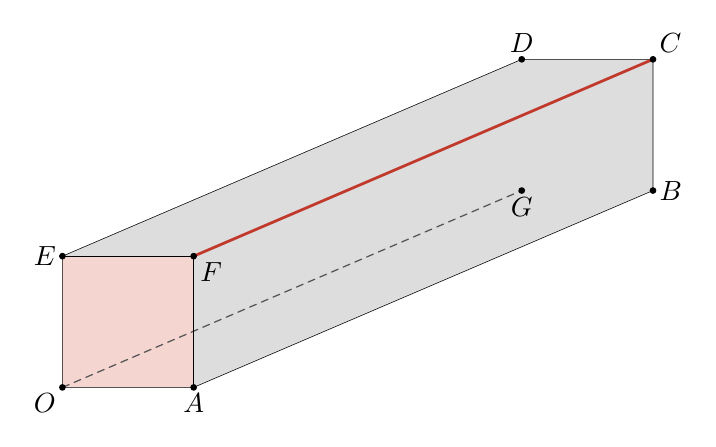
\begin{tikzpicture}
\tkzDefPoint(0.0,0.0){O} %! O = (0, 0)
\tkzDefPoint(1.6666667,0.0){A} %! A = (2, 0)
\tkzDefPoint(7.5000000,2.5000000){B} %! B = (9, 3)
\tkzDefPoint(7.5000000,4.1666667){C} %! C = (9, 5)
\tkzDefPoint(5.8333333,4.1666667){D} %! D = (7, 5)
\tkzDefPoint(0.0,1.6666667){E} %! E = (0, 2)
\tkzDefPoint(1.6666667,1.6666667){F} %! F = (2, 2)
\tkzDefPoint(5.8333333,2.5000000){G} %! G = (7, 3)
%! fact dist(A, F) == 2
%! fact dist(E, F) == 2
%! fact parallel(A, B, F, C)
%! fact parallel(E, D, F, C)
%! fact parallel(O, G, A, B)
%! fact parallel(A, F, B, C)
%! fact parallel(E, F, D, C)
\tkzFillPolygon[color=figaccenttint](O,A,F,E)
\tkzFillPolygon[color=figtint](A,B,C,F)
\tkzFillPolygon[color=figtint](E,F,C,D)
\tkzDrawSegment[aux](O,G)
\tkzDrawPolygon(O,A,B,C,D,E)
\tkzDrawSegment(A,F)
\tkzDrawSegment(E,F)
\tkzDrawSegment[key](F,C)
\tkzDrawPoints(O,A,B,C,D,E,F,G)
\tkzLabelPoint[below left,lbl](O){$O$}
\tkzLabelPoint[below,lbl](A){$A$}
\tkzLabelPoint[right,lbl](B){$B$}
\tkzLabelPoint[above right,lbl](C){$C$}
\tkzLabelPoint[above,lbl](D){$D$}
\tkzLabelPoint[left,lbl](E){$E$}
\tkzLabelPoint[below right,lbl](F){$F$}
\tkzLabelPoint[below,lbl](G){$G$}
\end{tikzpicture}
\end{document}
